\documentclass[a4paper, 11pt]{article}

\newcommand{\templates}{../../template}
\usepackage[a4paper, margin=2.5cm]{geometry}

\usepackage{enumitem}
\setlist[itemize]{noitemsep}
\setlist[enumerate]{noitemsep}

\let\oldpar\paragraph
\renewcommand{\paragraph}[1]{\oldpar{#1\\}\noindent}

% Avoid dots in the table of contents, it mess with the gulpease calculation
\makeatletter
\renewcommand{\@dotsep}{10000} 
\makeatother
\usepackage{graphicx}
\usepackage{hyperref}
\usepackage{makecell}
\usepackage{fancyhdr}

\newcommand{\settitolo}[1]{\newcommand{\titolo}{#1\\}}
\newcommand{\setprogetto}[1]{\newcommand{\progetto}{#1\\}}
\newcommand{\setcommittenti}[1]{\newcommand{\committenti}{#1\\}}
\newcommand{\setredattori}[1]{\newcommand{\redattori}{#1\\}}
\newcommand{\setrevisori}[1]{\newcommand{\revisori}{#1\\}}
\newcommand{\setresponsabili}[1]{\newcommand{\responsabili}{#1\\}}
\newcommand{\setversione}[1]{
	\ifdefined\versione\renewcommand{\versione}{#1\\}
	\else\newcommand{\versione}{#1\\}\fi
}
\newcommand{\setdestuso}[1]{\newcommand{\uso}{#1\\}}
\newcommand{\setdescrizione}[1]{\newcommand{\descrizione}{#1\\}}

\newcommand{\makefrontpage}{
	\begin{titlepage}
		\begin{center}

		
\includegraphics[width=0.4\textwidth]{\templates/4ourSquared_logo}\\

		{\Large 4OURSQUARED}\\[6pt]
		\href{mailto://4oursquared.unipd@gmail.com}{4oursquared.unipd@gmail.com}\\
		
		\ifdefined\progetto
		\vspace{1cm}
		{\Large\progetto}
		{\large\committenti}
		\else\fi
		
		\vspace{1.5cm}
		{\LARGE\titolo}
		
		\vfill
		
		\begin{tabular}{r | l}
		\multicolumn{2}{c}{\textit{Informazioni}}\\
		\hline
		
		\ifdefined\redattori
			\textit{Redattori} &
			\makecell[l]{\redattori}\\
		\else\fi
		\ifdefined\revisori
			\textit{Revisori} &
			\makecell[l]{\revisori}\\
		\else\fi
		\ifdefined\responsabili
			\textit{Responsabili} &
			\makecell[l]{\responsabili}\\
		\else\fi
		
		\ifdefined\versione
			\textit{Versione} & \versione
		\else\fi
		
		\textit{Uso} & \uso
		
		\end{tabular}
		
		\vspace{2cm}
		
		\ifdefined\descrizione
		Descrizione
		\vspace{6pt}
		\hrule
		\descrizione
		\else\fi
		\end{center}
	\end{titlepage}
}
\usepackage{hyperref}
\usepackage{array}
\usepackage{tabularx}
\usepackage{adjustbox}

\newcounter{verscount}
\setcounter{verscount}{0}
\newcommand{\addversione}[5]{
	\ifdefined\setversione
		\setversione{#1}
	\else\fi
	\stepcounter{verscount}
	\expandafter\newcommand%
		\csname ver\theverscount \endcsname{#1&#2&#3&#4&#5}
}

\newcommand{\listversioni}{
	\ifnum\value{verscount}>1
		\csname ver\theverscount \endcsname
		\addtocounter{verscount}{-1}
		\\\hline
		\listversioni
	\else
		\csname ver\theverscount \endcsname\\\hline
	\fi
}

\newcommand{\makeversioni}{
	\begin{center}
		\begin{tabularx}{\textwidth}{|c|c|c|c|X|}
		\hline
		\textbf{Versione} & \textbf{Data} & \textbf{Redattore} & \textbf{Verificatore} & \textbf{Descrizione} \\
		\hline
		\listversioni
		\end{tabularx}
	\end{center}
	\clearpage
}

\usepackage{longtable}
\usepackage{graphicx}
\usepackage{float}
\graphicspath{{img/}}

\settitolo{Specifica Tecnica}
\setprogetto{Lumos Minima}
\setcommittenti{Imola Informatica}
\setredattori{Soldà Matteo}
\setdestuso{esterno}
\setdescrizione{
Questo documento descrive la specifica architetturale del progetto, illustrando gli aspetti progettuali che caratterizzino il design del prodotto.
}

\addversione{0.0.0}{05/09/2023}{Soldà Matteo}{Alberti Nicolas}{Prima stesura.}
\addversione{0.0.1}{20/09/2023}{Soldà Matteo}{Alberti Nicolas}{Stesura delle prime sezioni.}
\addversione{0.0.2}{21/09/2023}{Soldà Matteo}{Alberti Nicolas}{Stesura delle parti mancanti esclusi dati relativi ai test}
\addversione{0.0.3}{22/09/2023}{Soldà Matteo}{Alberti Nicolas}{Stesura dei dati relativi ai test}
\addversione{0.1.0}{26/09/2023}{Alberti Nicolas}{Soldà Matteo}{Verifica per \textit{PB}}
\addversione{1.0.0}{26/09/2023}{Soldà Matteo}{Alberti Nicolas}{Approvazione per candidatura \textit{PB}}

\begin{document}
\makeindexdetails
\makefrontpage \makeversioni
\tableofcontents
\newpage
\listoffigures
\clearpage
\makecontentsdetails{Specifica Tecnica}
\newpage
\section{Introduzione}
\subsection{Scopo del Documento}
Questo documento ha lo scopo di descrivere nel dettaglio, sopratutto tramite diagrammi, le caratteristiche architetturali del prodotto software sviluppato.
\subsection{Riferimenti Normativi}
\begin{itemize}
    \item \href{https://www.math.unipd.it/~tullio/IS-1/2022/Progetto/C2.pdf}{Capitolato C2 - Lumos Minima}
\end{itemize}

\subsection{Riferimenti Informativi}
\begin{itemize}
    \item \href{https://www.math.unipd.it/~rcardin/swea/2022/Software%20Architecture%20Patterns.pdf}{Design Pattern Architetturali}
    \item \href{https://www.math.unipd.it/~rcardin/swea/2022/Design%20Pattern%20Architetturali%20-%20Dependency%20Injection.pdf}{Dependency Injection}
    \item \href{https://www.math.unipd.it/~rcardin/sweb/2022/L02.pdf}{MVC e Derivati}
    \item \href{https://www.math.unipd.it/~rcardin/swea/2022/Design%20Pattern%20Creazionali.pdf}{Pattern Creazionali}
    \item \href{http://www.math.unipd.it/~tullio/IS-1/2006/Approfondimenti/SEI-Software_Architectures.pdf}{Software Architecture}
    \item \href{https://www.math.unipd.it/~rcardin/swea/2022/Design%20Pattern%20Strutturali.pdf}{Pattern Strutturali}
    \item \href{https://www.math.unipd.it/~rcardin/swea/2021/Design%20Pattern%20Comportamentali_4x4.pdf}{Pattern Comportamentali}
    \item \href{https://www.math.unipd.it/~rcardin/swea/2021/SOLID%20Principles%20of%20Object-Oriented%20Design_4x4.pdf}{Programmazione SOLID}
\end{itemize}

\newpage
\section{Tecnologie Utilizzate}
\subsection{Frontend}
Per realizzare il frontend, ossia la parte di applicazione che viene eseguita sul browser dell'utente, sono state utilizzate le seguenti tecnologie:
\begin{itemize}
    \item React: libreria JavaScript per la creazione di interfacce utente;
    \item Typescript: linguaggio di programmazione che estende JavaScript aggiungendo i tipi, permettendo una codifica più robusta e sicura;
    \item Bootstrap: framework CSS per la creazione di interfacce responsive e accattivanti;
\end{itemize}
\subsection{Backend}
Per realizzare il backend, ossia la parte di applicazione che viene eseguita sul server, sono state utilizzate le seguenti tecnologie:
\begin{itemize}
    \item Node.js: runtime JavaScript che permette di eseguire codice JavaScript lato server;
    \item Typescript: linguaggio di programmazione che estende JavaScript aggiungendo i tipi, permettendo una codifica più robusta e sicura;
    \item Express: framework che permette di creare applicazioni web e API più facilmente e con una miglior gestione;
    \item Axios: client HTTP basato su promise per effettuare richieste HTTP basate su Promise;
    \item Mongoose: libreria che permette di gestire in modo più semplice e intuitivo i database MongoDB;
    \item Cors: middleware che permette di configurare in modo semplice e veloce le politiche CORS;
    \item JWT: libreria che permette di gestire in modo semplice e veloce i token JWT;
    \item Cron: libreria che permette di gestire in modo semplice e veloce i cronjob, ossia per la creazione di routine automatiche;
\end{itemize}

\subsection{Database}
Il database utilizzato è di tipo NoSQL, in particolare MongoDB, che permette di gestire documenti in formato BSON (Binary JSON).\\

\subsection{Meccanismo di Comunicazione}
Tutte le comunicazioni, sia esterne (da client a server) che interne (da server a server) sono state gestite tramite API REST.\\

\newpage
\section{Architettura Logica}
\subsection{Frontend}
\begin{figure}[H]
    \centering
    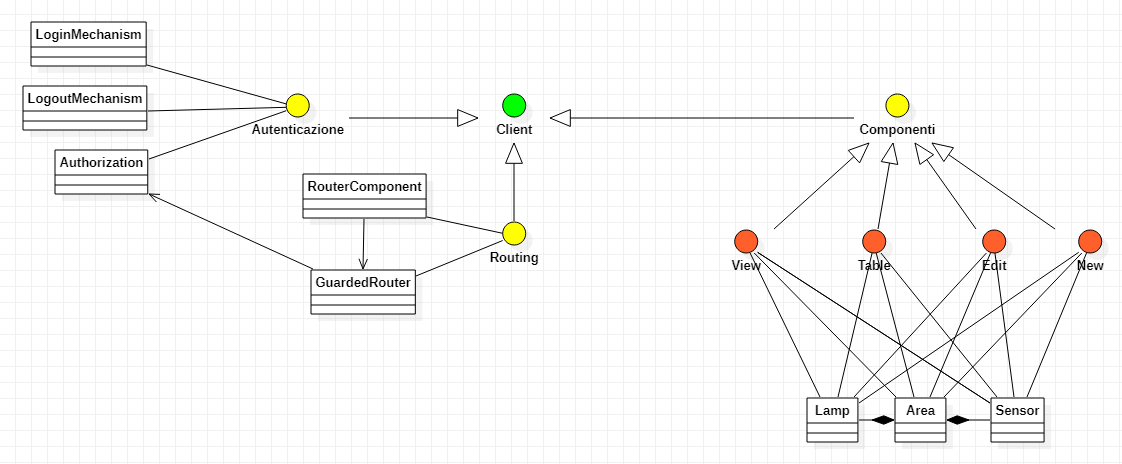
\includegraphics[width=\textwidth]{ArchitetturaClient}
    \caption{Architettura del client.}
\end{figure}
\subsection{Backend}
\begin{figure}[H]
    \centering
    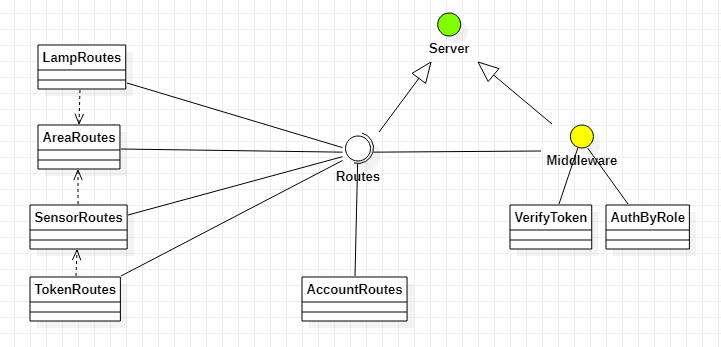
\includegraphics[width=\textwidth]{ArchitetturaServer}
    \caption{Architettura del server.}
\end{figure}

\newpage
\section{Design Pattern}
Lumos Minima è un'applicazione web di tipo SPA (Single-page application) per la gestione di impianti luminosi e di sensori per la rilevazione del movimento associati ai primi, raggruppati in insiemi definiti aree illuminate.\\
L'applicazione si avvale del cosiddetto stack MERN (dove le iniziali stanno rispettivamente per MongoDB, Express.JS, React.JS, Node.JS) e presenta un design architetturale “3-tier” dotata di un comparto client (presentazione), un server (“business logic”), e un database No-SQL per ospitare i dati (persistance). Tuttavia, invece di JavaScript “puro” si è preferito TypeScript, che viene compilato in JavaScript e fornisce un supporto opzionale della tipizzazione stretta. Il diagramma mostra le tecnologie di cui si serve ciascun layer.
\begin{figure}[H]
    \centering
    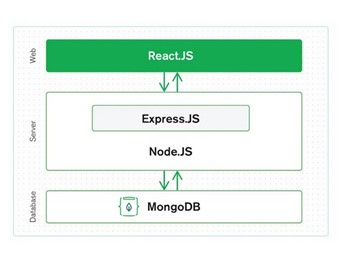
\includegraphics[width=\textwidth]{MERN}
    \caption{Rappresentazione grafica dell'architettura MERN.}
\end{figure}
Questo sistema “a livelli” è stato scelto poiché, oltre a trattarsi di un sistema consolidato (e quindi che si prestasse a uno sviluppo anche gravato da vincoli temporali stringenti), consente in modo agevole il mock del layer sottostante in occasione dei test di unità, vista la necessità di raggiungere la percentuale di code coverage inizialmente indicata nel capitolato.

\newpage
\section{Altri Aspetti Progettuali Rilevanti}
\subsection{Persistenza dei Dati}
Per realizzare lo strato di persistenza dei dati, come precedentemente indicato, è stato utilizzato MongoDB, un database NoSQL che permette di gestire documenti in formato BSON (Binary JSON).\\
\begin{figure}[H]
    \centering
    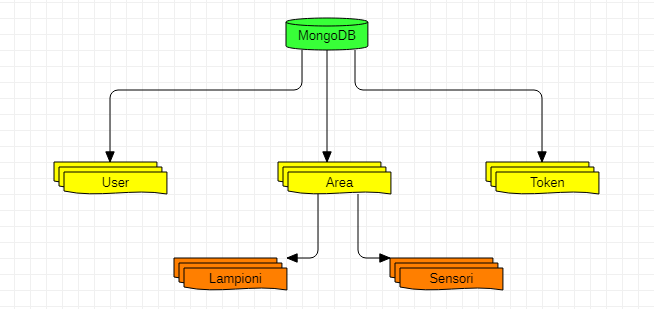
\includegraphics[width=\textwidth]{Persistenza}
    \caption{Struttura del database.}
\end{figure}
A differenza di un database di tipo SQL, in MongoDB, i dati sono raccolti in \textit{collezioni}. Queste \textit{collezioni} contengono uno, nessuno o una moltitudine di \textit{documenti}.\\
Dato che nei database di tipo NoSQL non esiste il concetto di "relazione", ogni documento di tipo area conterrà un array di documenti di tipo sensore e un array di documenti di tipo lampione.\\\\
Per quanto riguarda invece la comunicazione tra il server e il database, per poter comunicare i dati tra una parte e l'altra, sono stati utilizzati gli schemi di \textit{Mongoose} che permettevano di definire la struttura dei dati, i tipi di dati, i vincoli e le validazioni, oltre a fornire una interfaccia che permettesse di comunicare con il giusto tipo di dati.\\
Di seguito la struttura dei documenti (e conseguentemente degli schemi) utilizzati:
\begin{figure}[H]
    \centering
    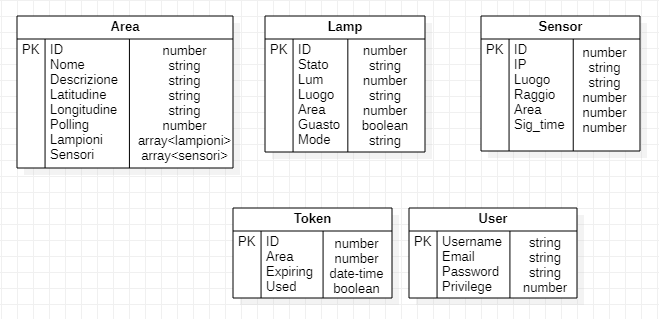
\includegraphics[width=\textwidth]{SchemaDB}
    \caption{Struttura dei dati nel DB.}
\end{figure}

\subsection{Interfacciamento tra Sensori e Lampioni}
Per accedere ai dati riguardanti un determinato lampione e/o sensore, abbiamo utilizzato la lettura di parametri dalla URL.\\ Ovviamente gli endpoint relativi ai sensori e ai lampioni sono distinti, infatti:
\begin{itemize}
    \item Endpoint sensori: \textit{/api/aree/$<$IdArea$>$/sensori/$<$IdSensore$>$};
    \item Endpoint lampioni: \textit{/api/aree/$<$IdArea$>$/lampioni/$<$IdLampione$>$};
\end{itemize}
\subsection{Comunicazione Automatica}
Per quanto riguarda il meccanismo che permette di aumentare e diminuire automaticamente la luminosità dei lampioni che si trovano dentro una determinata area illuminata, il soggetto principale sono i sensori: essi, qualora rilevassero il movimento di una persona, di un veicolo o di un animale, dovrebbero inviare una richiesta di tipo HTTP all'endpoint prestabilito. Alla ricezione della richiesta, il server si occuperà della gestione della stessa come descritto nel diagramma sottostante.
\begin{figure}[H]
    \centering
    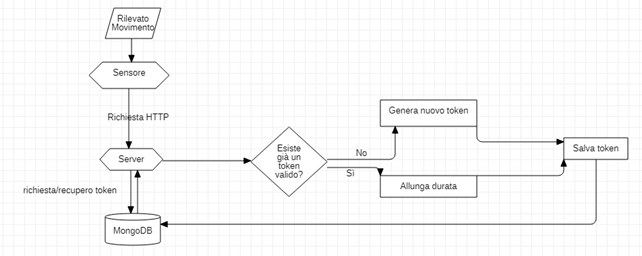
\includegraphics[width=\textwidth]{sensori}
    \caption{Diagramma di flusso del segnale relativo al movimento rilevato dai sensori.}
\end{figure}
Il token trova un utilizzo concreto solo per i lampioni dell'area che sono configurati in modalità PULL (manuale).\\
Per questo motivo, di seguito c'è una piccola spiegazione di come viene gestito il rilevamento di movimento da entrambi i tipi di lampione:
\begin{itemize}
    \item PUSH: i lampioni si illuminano quando il sensore segnala un movimento, senza necessità di utilizzare il token
    \item PULL: la parte di server vhe gestisce l'area illuminata, con cadenza regolare e definita dall'attributo \textit{polling time}, controlla nel database se c'è un token valido per l'area di riferimento:
          \begin{itemize}
              \item Se il token è valido e inutilizzato: illumina tutti i lampioni impostati in modalità PULL;
              \item Se il token non è valido ma è stato utilizzato: riduce la luminosità di tutti i lampioni a quella iniziale;
              \item Negli altri casi, verrà restituito un codice stato consono, ma senza effettuare nessun'altra azione.
          \end{itemize}
\end{itemize}

\subsection{Autenticazione e Autorizzazione tramite JWT}
Dopo aver inserito le proprie credenziali nella login mask, se la password (criptata con hashing SHA512) coincide con quella dell'utente viene restituito un token JWT firmato dal server, una stringa che contiene informazioni sul ruolo dell'utente. L'autorizzazione (necessaria per l'accesso alle pagine dal lato “client”, e per utilizzare le API del server) sfrutta questo meccanismo:
\begin{figure}[H]
    \centering
    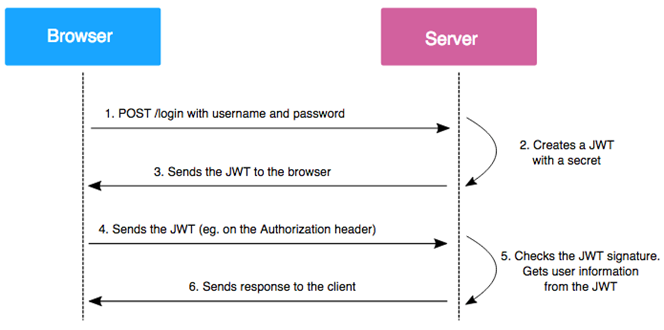
\includegraphics[width=\textwidth]{auth}
    \caption{Diagramma di flusso del meccanismo di autorizzazione tramite JWT.}
\end{figure}

Tuttavia, il JWT è memorizzato (e inviato al server) all'interno di un cookie HTTP-Only: questo impedisce che il contenuto del cookie possa essere letto da codice JavaScript malevolo, vanificando così attacchi alla confidenzialità di tipo XSS (Cross-Site Scripting).\\\\
Le API sono protette da due livelli di middleware che prendono in carico la richiesta HTTP.
\begin{figure}[H]
    \centering
    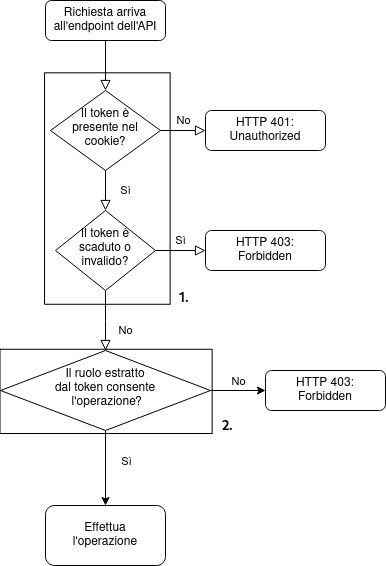
\includegraphics[width=\textwidth]{middleware}
    \caption{Diagramma di flusso del meccanismo di autorizzazione tramite middleware.}
\end{figure}

\subsection{Client e Smart Components}
Il layer di presentazione in React.JS adopera Smart, o “Stateful” Components, ovvero dei moduli - uno per ciascun macro-elemento dell'app - aventi come responsabilità, oltre al semplice rendering a schermo, la gestione di uno stato interno. Questa scelta si presta alla naive hierarchical architecture (S. Nelson):
\begin{itemize}
    \item Quando richiesto dall'utente, avviene un render iniziale del componente;
    \item In maniera asincrona (non bloccante), i dati vengono quindi reperiti dal business layer tramite lo “hook” useEffect;
    \item Nello hook, i dati appena reperiti vengono immessi nello stato locale con la funzione setState: ciò comporta un re-render che mostrerà tali dati;
    \item In presenza di un input dell'utente viene trasmessa la modifica al business layer, e (qualora questa abbia successo) in concomitanza avviene l'aggiornamento “locale” dello stato del componente con la stessa funzione setState, che ne comporta così un re-render che rispecchia la modifica.
\end{itemize}
\begin{figure}[H]
    \centering
    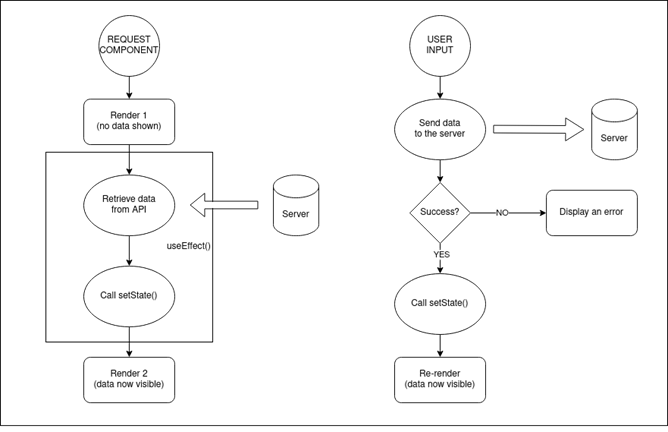
\includegraphics[width=\textwidth]{SmartComponent}
    \caption{Diagramma di flusso del meccanismo di re-render.}
\end{figure}

\subsection{Sicurezza}
Per assicurarsi di evitare gravi problemi legati alla sicurezza, sono stati implementati dei moduli all'interno di \textit{GitHub} che ad ogni \textit{push} o \textit{pull request} controllano che il codice sia conforme a determinati standard.\\
Gli strumenti utilizzati sono stati:
\begin{itemize}
    \item Snyk
    \item SonarCloud
    \item GitHub CodScanning
\end{itemize}
Prima di poter effettuare il merge nei branch \textit{dev} (relativo allo sviluppo) oppure nel branch \textit{main} (relativo alle versioni stabili del prodotto), era necessario che tutti i controlli venissero superati, che non fosse presente una duplicazione del codice superiore al $3\%$ e che non fossero presenti \textit{code smells}.\\
\section{Requisiti e Soddisfacimento}
\subsection{Tabella dei Requisiti}
\setlength\tabcolsep{4pt}
\begin{longtable}{|c|p{7cm}|c|p{4cm}|}
    \hline
    \multicolumn{4}{| c |}{\textbf{Requisiti funzionali}}                                                                                                                                                                       \\
    \hline
    \textbf{Codice} & \textbf{Descrizione}                                                                                                                                          & \textbf{Rilevanza} & \textbf{Soddisfatto} \\
    \hline
    RF1-O           & Rilevamento della presenza di individui in una delle aree illuminate.                                                                                         & Obbligatorio       & SI                   \\
    \hline
    RF2-O           & Acquisizione dell'intensità luminosa e successiva determinazione precisa del livello di luminosità.                                                           & Obbligatorio       & SI                   \\
    \hline
    RF3-O           & Una volta acquisito il livello di luminosità iniziale, l'operatore autenticato aumenta manualmente il livello di intesità luminosa.                           & Obbligatorio       & SI                   \\
    \hline
    RF4-O           & Una volta acquisito il livello di luminosità iniziale, l'operatore autenticato diminuisce manualmente il livello di intensità luminosa.                       & Obbligatorio       & SI                   \\
    \hline
    RF5-O           & Il gestore può effettuare l'accesso per gestire manualmente i sistemi di illuminazione.                                                                       & Obbligatorio       & SI                   \\
    \hline
    RF6-O           & Il gestore può effettuare il logout dall'interno dell'area di gestione dei sistemi.                                                                           & Obbligatorio       & SI                   \\
    \hline
    RF7-O           & Il gestore può consultare l'intero elenco delle aree illuminate.                                                                                              & Obbligatorio       & SI                   \\
    \hline
    RF8-O           & Il gestore può consultare l'intero elenco delle aree illuminate con guasti.                                                                                   & Obbligatorio       & SI                   \\
    \hline
    RF9-O           & Il gestore può aggiungere manualmente un guasto selezionando un impianto dalla lista di quelli attivi.                                                        & Obbligatorio       & SI                   \\
    \hline
    RF10-O          & Il gestore può creare una nuova area illuminata, inserendone la posizione geografica e i relativi dettagli.                                                   & Obbligatorio       & SI                   \\
    \hline
    RF11-O          & Il gestore può modificare i dettagli di un'area illuminata già esistente.                                                                                     & Obbligatorio       & SI                   \\
    \hline
    RF12-O          & Il gestore può rimuovere un'area illuminata già esistente.                                                                                                    & Obbligatorio       & SI                   \\
    \hline
    RF13-O          & Il sistema di gestione dell'illuminazione aumenta l'intensità luminosa al passaggio di una o più persone.                                                     & Obbligatorio       & SI                   \\
    \hline
    RF14-O          & Il sistema di gestione dell'illuminazione diminuisce l'intensità luminosa al passaggio di una o più persone.                                                  & Obbligatorio       & SI                   \\
    \hline
    RF15-O          & Il gestore può impostare la modalità di funzionamento automatico per l'impianto selezionato.                                                                  & Obbligatorio       & SI                   \\
    \hline
    RF16-O          & Il gestore può rimuovere un'area illuminata dall'elenco delle aree illuminate con guasti e ritorna nelle aree illuminate attive.                              & Obbligatorio       & SI                   \\
    \hline
    RF17-O          & Inserimento di un nuovo sensore in un'area per essere gestito dal sistema.                                                                                    & Obbligatorio       & SI                   \\
    \hline
    RF18-O          & Il gestore può rimuovere dal sistema uno dei sensori registrati.                                                                                              & Obbligatorio       & SI                   \\
    \hline
    RF19-O          & Il gestore può inserire nel sistema l'impianto di illuminazione da attivare con i relativi dettagli.                                                          & Obbligatorio       & SI                   \\
    \hline
    RF20-O          & Il gestore può rimuovere dal sistema uno degli impianti luminosi registrati.                                                                                  & Obbligatorio       & SI                   \\
    \hline
    RF21-O          & Rilevamento della presenza di individui in modalità automatica in una delle aree illuminate                                                                   & Obbligatorio       & SI                   \\
    \hline
    RF22-F          & Rilevamento della presenza di individui su richiesta in una delle aree illuminate                                                                             & Facoltativo        & SI                   \\
    \hline
    RF23-O          & Una volta acquisito il livello di luminosità iniziale, l'operatore autenticato aumenta manualmente il livello di intensità luminosa di un'area illuminata     & Obbligatorio       & SI                   \\
    \hline
    RF24-F          & Una volta acquisito il livello di luminosità iniziale, l'operatore autenticato aumenta manualmente il livello di intensità luminosa di più aree illuminate    & Facoltativo        & NO                   \\
    \hline
    RF25-O          & Una volta acquisito il livello di luminosità iniziale, l'operatore autenticato diminuisce manualmente il livello di intensità luminosa di un'area illuminata  & Obbligatorio       & SI                   \\
    \hline
    RF26-F          & Una volta acquisito il livello di luminosità iniziale, l'operatore autenticato diminuisce manualmente il livello di intensità luminosa di più aree illuminate & Facoltativo        & NO                   \\
    \hline
    RF27-O          & Una volta acquisito il livello di luminosità iniziale, il sistema aumenta automaticamente il livello di intensità luminosa di un'area illuminata              & Obbligatorio       & SI                   \\
    \hline
    RF28-F          & Una volta acquisito il livello di luminosità iniziale, il sistema aumenta automaticamente il livello di intensità luminosa di più aree illuminate             & Facoltativo        & NO                   \\
    \hline
    RF29-O          & Una volta acquisito il livello di luminosità iniziale, il sistema diminuisce automaticamente il livello di intensità luminosa di un'area illuminata           & Obbligatorio       & SI                   \\
    \hline
    RF30-F          & Una volta acquisito il livello di luminosità iniziale, il sistema diminuisce automaticamente il livello di intensità luminosa di più aree illuminate          & Facoltativo        & NO                   \\
    \hline
    RF31-F          & Una volta rilevato un valore di intensità luminosa sotto soglia, il sistema provvede ad aumentare l'intensità luminosa.                                       & Facoltativo        & NO                   \\
    \hline
    RF32-F          & Una volta rilevato un valore di intensità luminosa sopra soglia, il sistema provvede ad diminuire l'intensità luminosa.                                       & Facoltativo        & NO                   \\
    \hline
    RF33-F          & Il sensore rileva un'intensità luminosa che è sopra un certo valore soglia.                                                                                   & Facoltativo        & NO                   \\
    \hline
    RF34-F          & Il sensore rileva un'intensità luminosa che è sotto un certo valore soglia.                                                                                   & Facoltativo        & NO                   \\
    \hline
    RF35-F          & Il sistema rileva la presenza di un guasto o un'anomalia riguardo una misurazione errata.                                                                     & Facoltativo        & NO                   \\
    \hline
    RF36-F          & Il sistema provvede ad inserire nella lista di impianti guasti l'area in cui è presente l'anomalia.                                                           & Facoltativo        & NO                   \\
    \hline
    RF37-F          & Durante l'inserimento di un nuovo sensore si specifica il tipo di interazione automatico (push) con il sistema.                                               & Facoltativo        & SI                   \\
    \hline
    RF38-F          & Durante l'inserimento di un nuovo sensore si specifica il tipo di interazione su richiesta (pull) con il sistema.                                             & Facoltativo        & SI                   \\
    \hline
    RF39-O          & Durante l'inserimento di un nuovo sensore si specificano i dettagli relativi a tale sensore.                                                                  & Obbligatorio       & SI                   \\
    \hline
    RF40-O          & Durante l'inserimento di un nuovo sensore si specifica la posizione geografica del sensore di riferimento.                                                    & Obbligatorio       & SI                   \\
    \hline
    RF41-O          & Durante l'inserimento di un nuovo sensore si specifica l'ampiezza del raggio d'azione del sensore che si sta aggiungendo.                                     & Obbligatorio       & SI                   \\
    \hline
    RF42-O          & L'impianto guasto viene riparato dal Manutentore e viene segnalato come nuovamente funzionante.                                                               & Obbligatorio       & SI                   \\
    \hline
\end{longtable}
Tutti i requisiti funzionali obbligatori sono stati soddisfatti. I requisiti funzionali facoltativi sono stati soddisfatti in parte, in quanto non sono stati implementati i requisiti facoltativi che riguardano la gestione di più aree illuminate contemporaneamente a causa del poco tempo rimanente, anche se oggettivamente sarebbero di facile implementazione.\\




\subsection{Requisiti di Qualità}
\setlength\tabcolsep{4pt}
\begin{longtable}{|c|p{7cm}|c|p{4cm}|}
    \hline
    \multicolumn{4}{| c |}{\textbf{Requisiti di Qualità}}                                                                                                                                                       \\
    \hline
    \textbf{Codice} & \textbf{Descrizione}                                                                                                                          & \textbf{Rilevanza} & \textbf{Soddisfatto} \\
    \hline
    RQ1-O           & Test che dimostrino il corretto funzionamento dei servizi e delle funzionalità previste, con una copertura dell'70\% del codice.              & Obbligatorio       & SI                   \\
    \hline
    RQ2-O           & Documenti su scelte implementative e progettuale e relative motivazioni, i problemi aperti e le eventuali soluzioni proposte da approfondire. & Obbligatorio       & SI                   \\
    \hline
    RQ3-O           & Web Application responsive per soddisfare i requisiti obbligatori nei casi d'uso.                                                             & Obbligatorio       & SI                   \\
    \hline
\end{longtable}
Tutti i requisiti di qualità, in quanto obbligatori, sono stati soddisfatti.\\

\subsection{Code Coverage}
I moduli utilizzati per la code coverage sono stati:
\begin{itemize}
    \item \textbf{Jest}: framework per l'esecuzione di test JavaScript;
    \item \textbf{Supertest}: framework per l'esecuzione di test HTTP;
\end{itemize}

Inoltre, per verificare la duplicazione di codice è stato utilizzato \textbf{SonarCloud}.\\
Con il committente, inizialmente era stata richiesta una percentuale minima dell'$80\%$, ma in seguito agli incontri di presentazione, riconoscendo che il codice è altamente modulare, è stata abbassata al $70\%$ così da poter escludere costruttori, distruttori e funzioni di supporto raramente utilizzate ma comunque utili.\\
I test sono riproducibili tramite il comando \textit{npm run coverage} dentro la
directory \textit{/client}, mentre con il comando \textit{npm test} dentro la directory \textit{/server} per i test relativi al frontend
e al backend. Le percentuali riportate indicano la media, che viene riportata
nella prima riga del report.\\

\begin{figure}[H]
    \centering
    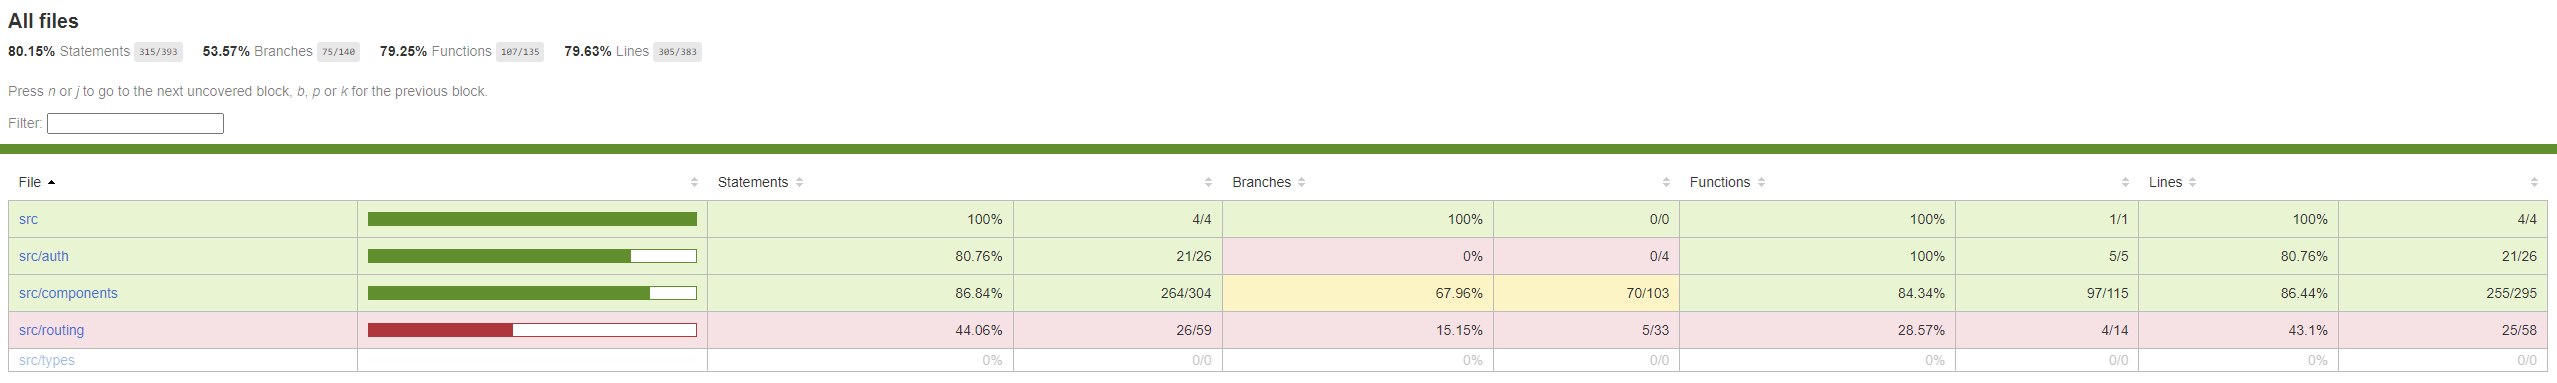
\includegraphics[width=\textwidth]{test_client}
    \caption{Code coverage del frontend.}
\end{figure}

\begin{figure}[H]
    \centering
    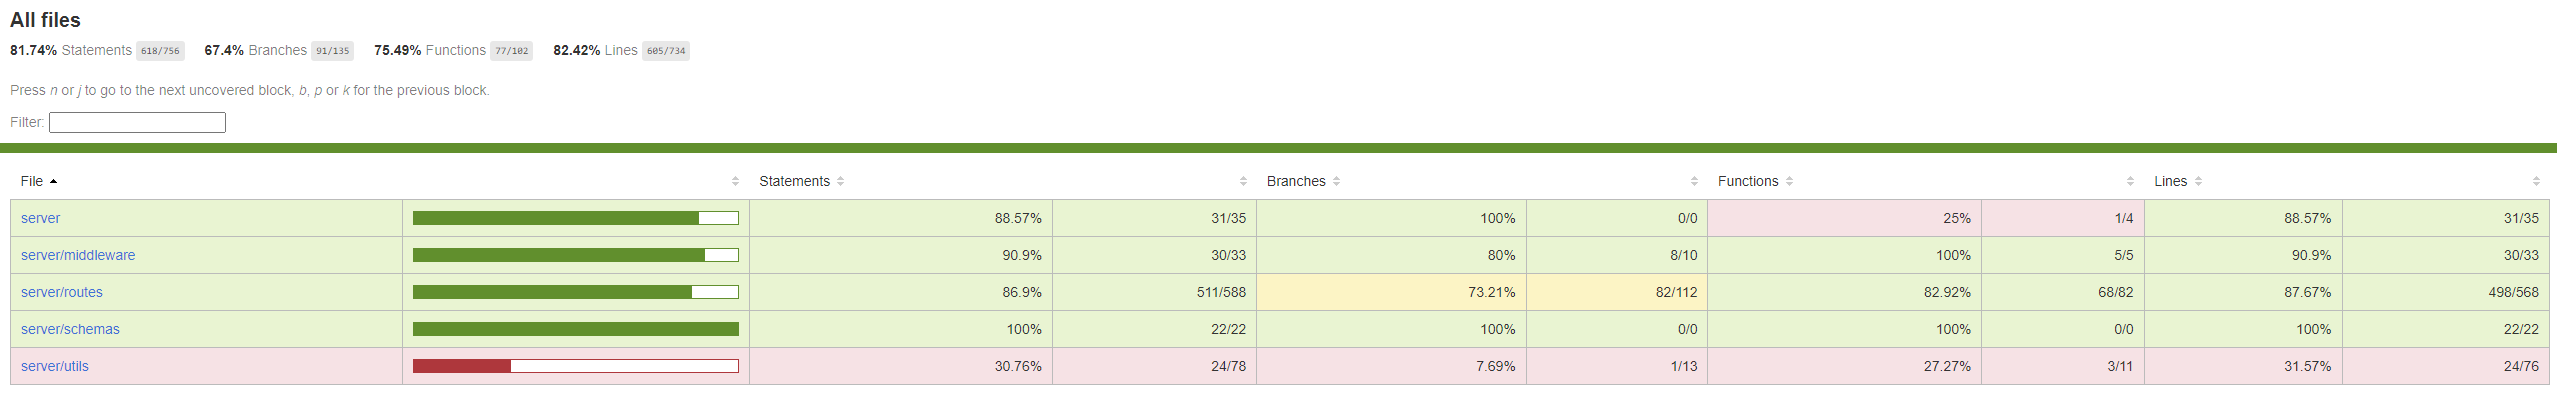
\includegraphics[width=\textwidth]{test-server}
    \caption{Code coverage del backend.}
\end{figure}

\end{document}